% !TeX root = ../main.tex
\chapter{Insiemi e operazioni}
\fonti{Lezioni 1, 2 e 3}

\section{Operazioni tra insiemi}
% Fonti: L1 pp. 1--3; L2 pp. 1--2; L3 pp. 1--2.
Per dimostrare che due insiemi sono uguali si possono provare le due inclusioni, oppure verificare che ogni elemento appartiene al primo se e solo se appartiene al secondo. Tutte le operazioni seguenti sono descritte attraverso questo criterio di appartenenza.

\begin{definizione}
Siano $A$ e $B$ insiemi. Si definiscono
\[
\begin{aligned}
A\cup B&=\{x\mid x\in A\ \text{oppure}\ x\in B\},\\
A\cap B&=\{x\mid x\in A\ \text{e}\ x\in B\},\\
A\setminus B&=\{x\mid x\in A\ \text{e}\ x\notin B\},\\
A\mathbin\triangle B&=(A\setminus B)\cup(B\setminus A).
\end{aligned}
\]
L'ultima operazione si chiama \textbf{differenza simmetrica}: un elemento vi appartiene esattamente quando appartiene a uno solo dei due insiemi. Due insiemi si dicono \textbf{disgiunti} se $A\cap B=\varnothing$.
\end{definizione}

\begin{schema}
\begin{tikzpicture}[scale=.67]
  \foreach \t/\lab in {0/Unione,4.5/Intersezione,9/Differenza,13.5/Diff. simmetrica}{
    \begin{scope}[shift={(\t,0)}]
      \ifdim\t pt=0pt\relax\fill[coloreschema!18] (0,0) circle (1);\fill[coloreschema!18] (1.2,0) circle (1);\fi
      \ifdim\t pt=4.5pt\relax\begin{scope}\clip (0,0) circle (1);\fill[coloreschema!18] (1.2,0) circle (1);\end{scope}\fi
      \ifdim\t pt=9pt\relax\begin{scope}\clip (0,0) circle (1);\fill[coloreschema!18] (-1,-1) rectangle (2.3,1);\fill[white] (1.2,0) circle (1);\end{scope}\fi
      \ifdim\t pt=13.5pt\relax\fill[coloreschema!18,even odd rule] (0,0) circle (1) (1.2,0) circle (1);\fi
      \draw (0,0) circle (1);\draw (1.2,0) circle (1);
      \node at (-.35,.5) {$A$};\node at (1.55,.5) {$B$};\node at (.6,-1.5) {\lab};
    \end{scope}
  }
\end{tikzpicture}
\end{schema}

\begin{proposizione}
Unione e intersezione sono commutative e associative. Inoltre
\[
A\mathbin\triangle B=(A\cup B)\setminus(A\cap B),
\]
e la differenza simmetrica è commutativa.
\end{proposizione}
\begin{proof}
La condizione «$x\in A$ oppure $x\in B$» non cambia scambiando $A$ e $B$; lo stesso vale per «e». Le due condizioni con tre insiemi, «appartiene ad almeno uno» e «appartiene a tutti», non dipendono dalle parentesi: questo prova l'associatività.

Per la differenza simmetrica, appartenere a uno solo dei due insiemi equivale ad appartenere alla loro unione senza appartenere alla loro intersezione. La condizione è simmetrica in $A$ e $B$.
\end{proof}

\begin{esercizio}[Associatività della differenza]
Stabilire se la differenza e la differenza simmetrica siano associative.
\end{esercizio}
\begin{svolgimento}
\textbf{Differenza.} Non è associativa. Ponendo $A=B=C=\{0\}$ si ha
\[
(A\setminus B)\setminus C=\varnothing,
\qquad A\setminus(B\setminus C)=\{0\}.
\]
Non è neppure commutativa: $\{0\}\setminus\varnothing=\{0\}$, mentre $\varnothing\setminus\{0\}=\varnothing$.

\textbf{Differenza simmetrica.} Confrontiamo direttamente i due membri attraverso le operazioni già definite. Poniamo
\[
\begin{aligned}
A_0&=A\setminus(B\cup C),& B_0&=B\setminus(A\cup C),\\
C_0&=C\setminus(A\cup B),& T&=A\cap B\cap C,
\end{aligned}
\]
\passomath{(A\triangle B)\triangle C} Per definizione è l'unione di $(A\triangle B)\setminus C$ e $C\setminus(A\triangle B)$. Il primo insieme contiene i punti che stanno in uno solo fra $A,B$ e sono esterni a $C$; il secondo contiene i punti di $C$ che sono esterni sia ad $A$ sia a $B$, oppure appartengono a entrambi. Dunque
\[
(A\triangle B)\setminus C=A_0\cup B_0,
\qquad C\setminus(A\triangle B)=C_0\cup T.
\]
\passomath{A\triangle(B\triangle C)} Questa volta i due pezzi della definizione sono $A\setminus(B\triangle C)$ e $(B\triangle C)\setminus A$. Il primo contiene i punti di $A$ che sono esterni sia a $B$ sia a $C$, oppure appartengono a entrambi; il secondo contiene i punti esterni ad $A$ che stanno in uno solo fra $B,C$. Pertanto
\[
A\setminus(B\triangle C)=A_0\cup T,
\qquad (B\triangle C)\setminus A=B_0\cup C_0.
\]
Per commutatività e associatività dell'unione, già dimostrate, i due membri coincidono con $A_0\cup B_0\cup C_0\cup T$. Questo prova l'associatività senza usare strumenti ulteriori.
\end{svolgimento}

\begin{schema}
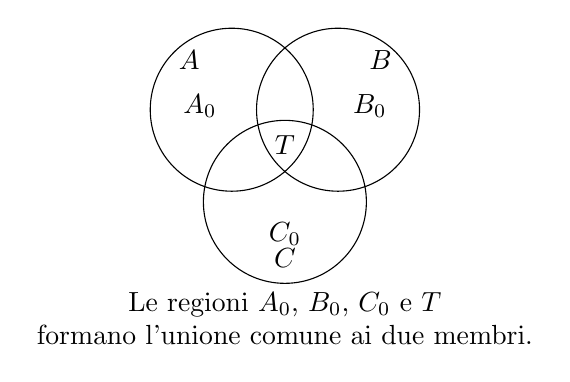
\begin{tikzpicture}[scale=.9]
  \draw (0,.45) circle (1.15);\draw (1.5,.45) circle (1.15);\draw (.75,-.85) circle (1.15);
  \node at (-.6,1.15) {$A$};\node at (2.1,1.15) {$B$};\node at (.75,-1.65) {$C$};
  \node at (-.45,.5) {$A_0$};\node at (1.95,.5) {$B_0$};\node at (.75,-1.3) {$C_0$};\node at (.75,-.05) {$T$};
  \node[align=center] at (.75,-2.5) {Le regioni $A_0$, $B_0$, $C_0$ e $T$\\formano l'unione comune ai due membri.};
\end{tikzpicture}
\end{schema}

\section{Famiglie di insiemi e insieme delle parti}
\begin{definizione}
Una \textbf{famiglia indicizzata} di insiemi è una famiglia $(A_i)_{i\in I}$, dove $I$ è l'insieme degli indici. Si pone
\[
\bigcup_{i\in I}A_i=\{x\mid \exists i\in I:\ x\in A_i\},
\qquad
\bigcap_{i\in I}A_i=\{x\mid \forall i\in I:\ x\in A_i\}.
\]
Per l'intersezione assumiamo $I\ne\varnothing$, oppure fissiamo un ambiente $X$ contenente tutti gli $A_i$: in tale ambiente l'intersezione della famiglia vuota è $X$. L'unione della famiglia vuota è $\varnothing$.
\end{definizione}

\begin{definizione}
L'\textbf{insieme delle parti} di $X$ è
\[
\mathcal P(X)=\{A\mid A\subseteq X\}.
\]
Per $A\subseteq X$, il \textbf{complementare} di $A$ in $X$ è $A^c=X\setminus A$; si usa anche la notazione $C(A)$. Vale $(A^c)^c=A$.
\end{definizione}

\begin{schema}
\begin{tikzpicture}[scale=.75]
  \fill[coloreschema!16] (0,0) rectangle (4.5,2.4);\fill[white] (1.5,1.2) circle (.8);
  \draw (0,0) rectangle (4.5,2.4);\draw (1.5,1.2) circle (.8);
  \node at (1.5,1.2) {$A$};\node at (3.3,1.2) {$A^c$};\node[above right] at (4.5,2.2) {$X$};
\end{tikzpicture}
\end{schema}

\begin{esempio}
Se $X=\{2,3,4\}$, allora
\[
\mathcal P(X)=\{\varnothing,\{2\},\{3\},\{4\},\{2,3\},\{2,4\},\{3,4\},X\}.
\]
In particolare $\varnothing\in\mathcal P(X)$ e $X\in\mathcal P(X)$: appartenenza e inclusione sono concetti diversi.
\end{esempio}

\begin{proposizione}[Leggi di De Morgan e distributività]
Per $A,B,C\subseteq X$ si ha
\[
\begin{aligned}
(A\cup B)^c&=A^c\cap B^c,&(A\cap B)^c&=A^c\cup B^c,\\
(A\cup B)\cap C&=(A\cap C)\cup(B\cap C),\\
(A\cap B)\cup C&=(A\cup C)\cap(B\cup C),\\
(A\triangle B)\cap C&=(A\cap C)\triangle(B\cap C).
\end{aligned}
\]
\end{proposizione}
\begin{proof}
\textbf{Complementi.} Per $x\in X$, non appartenere ad $A\cup B$ significa non appartenere né ad $A$ né a $B$; non appartenere ad $A\cap B$ significa che almeno una delle due appartenenze è falsa. Sono precisamente le due identità di De Morgan.

\textbf{Distributività.} La condizione $(x\in A\ \text{oppure}\ x\in B)$ e $x\in C$ equivale a $(x\in A\ \text{e}\ x\in C)$ oppure $(x\in B\ \text{e}\ x\in C)$. Per la seconda identità, se $x\in C$ appartiene a entrambi i membri; se $x\notin C$, entrambi richiedono $x\in A\cap B$.

\textbf{Differenza simmetrica.} Se $x\notin C$, non appartiene a nessuno dei due membri. Se $x\in C$, entrambi richiedono che appartenga a uno solo tra $A$ e $B$.
\end{proof}

Il controllo si può tradurre in tabelle di verità: fissato $x\in X$, si assegnano V o F alle proposizioni di appartenenza. Per esempio, la prima legge di De Morgan corrisponde alla tabella
\[
\begin{array}{cc|c|c}
x\in A&x\in B&x\in(A\cup B)^c&x\in A^c\cap B^c\\\hline
\mathrm V&\mathrm V&\mathrm F&\mathrm F\\
\mathrm V&\mathrm F&\mathrm F&\mathrm F\\
\mathrm F&\mathrm V&\mathrm F&\mathrm F\\
\mathrm F&\mathrm F&\mathrm V&\mathrm V
\end{array}
\]

\begin{esercizio}[Elementi neutri e possibilità di annullamento]
Nell'insieme $\mathcal P(X)$ verificare $A\triangle\varnothing=A$ e $A\cap X=A$. Dato $A$, esiste $B$ con $A\triangle B=\varnothing$? Per quali $A$ esiste $B$ con $A\cap B=X$?
\end{esercizio}
\begin{svolgimento}
La differenza simmetrica con l'insieme vuoto conserva esattamente gli elementi di $A$; l'intersezione con $X$ conserva ogni elemento di $A\subseteq X$.

Si ha $A\triangle B=\varnothing$ se e solo se non esistono elementi in uno solo dei due insiemi, cioè se e solo se $A=B$. Dunque $B=A$ è l'unica soluzione.

Da $A\cap B=X$ e $A,B\subseteq X$ segue $X\subseteq A\subseteq X$ e $X\subseteq B\subseteq X$, quindi necessariamente $A=B=X$. Viceversa questa scelta funziona. Per $X\ne\varnothing$ non tutti gli elementi di $\mathcal P(X)$ ammettono quindi un tale $B$.
\end{svolgimento}

\section{Prodotti cartesiani}
% Fonte: L1 pp. 3--4.
\begin{definizione}
Il \textbf{prodotto cartesiano} di $A$ e $B$ è l'insieme delle coppie ordinate
\[
A\times B=\{(a,b)\mid a\in A,\ b\in B\}.
\]
L'ordine conta: $(a,b)=(a',b')$ se e solo se $a=a'$ e $b=b'$. Per un numero finito di fattori,
\[
A_1\times\cdots\times A_n=\{(x_1,\ldots,x_n)\mid x_i\in A_i\ \text{per ogni }i\}.
\]
Quando tutti i fattori coincidono con $A$, si scrive $A^n$. In particolare $\R^2=\R\times\R$.
\end{definizione}

\begin{esempio}
Per $A=\{m,n,p\}$ e $B=\{9,8\}$,
\[
A\times B=\{(m,9),(m,8),(n,9),(n,8),(p,9),(p,8)\}.
\]
Il prodotto è vuoto se almeno un fattore è vuoto. In generale $A\times B$ e $B\times A$ non sono lo stesso insieme; la corrispondenza $(a,b)\mapsto(b,a)$ scambia però biunivocamente le coppie.
\end{esempio}
